得益于量子叠加、量子纠缠和量子并行性等原理，量子算法能够高效处理某些计算问题，例如 Shor 算法 \cite{shor1994algorithms}、Grover 算法 \cite{grover1996fast,long2001grover} 和 Harrow-Hassidim-Lloyd 算法 \cite{harrow2009quantum}，并相较经典算法实现指数级或多项式级加速。然而，当前阶段的量子设备仍受限于量子比特数量有限和显著噪声，通常称为含噪中等规模量子（NISQ）设备 \cite{preskill2018quantum}。需要注意的是，上述量子算法在 NISQ 时代并不表现出量子优势。

变分量子算法（Variational Quantum Algorithms, VQA）\cite{cerezo2021variational,yuan2019theory,xu2021variational} 被认为是 NISQ 时代实现量子优势最有希望的候选方案。VQA 利用经典机器学习中的优化算法，对参数化量子线路（Parameterized Quantum Circuit, PQC）进行调优。因此，VQA 是一种量子-经典混合算法。VQA 已广泛应用于多个领域，包括量子多体模拟 \cite{Peruzzo2014Peruzzo2014,kandala2017hardware,kokail2019self,lyu2023variational,Lyu2023symmetryenhanced,cao2022progress}、量子近似优化算法 \cite{farhi2014quantum,patti2022variational,chandarana2023digitized}、量子机器学习 \cite{benedetti2019parameterized,wei2022quantum,lloyd2018quantum,biamonte2017quantum,abbas2021power} 和纠缠纯化 \cite{zhang2023variational}。本节将简要概述 VQA 算法的工作流程，以及如何在 \MindQuantum\ 中高效实现该流程。更多 VQA 算法应用示例将在第 \ref{sec:applications} 章中展示。

\begin{figure}[h]
  \begin{center}
    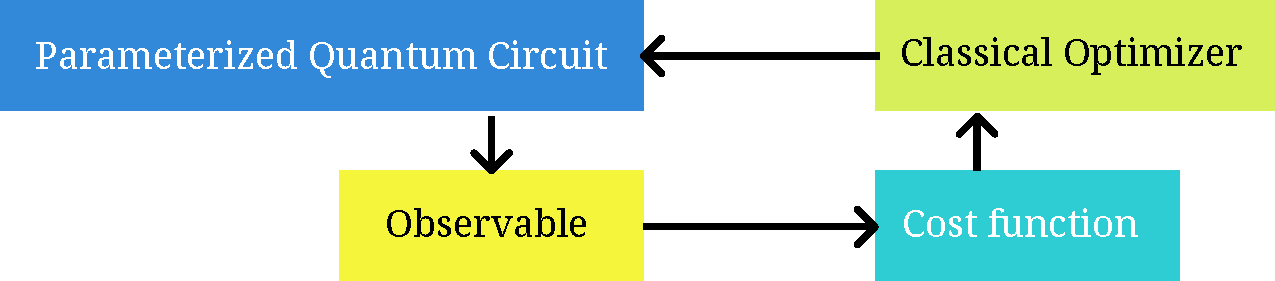
\includegraphics[width=0.9\linewidth]{images/4_1_vqa.pdf}
  \end{center}
  \caption{VQA 的工作流程。}
  \label{fig:vqa_work_flow}
\end{figure}

图~\ref{fig:vqa_work_flow} 展示了 VQA 的主要工作流程。VQA 的核心组成部分是 PQC，其中既包含 Hadamard 门和 Pauli 门等非参数化量子门，也包含绕 Bloch 球 $x$、$y$ 或 $z$ 轴旋转的参数化量子门。根据具体任务，PQC 可以分为两部分：编码器线路负责将经典数据编码为量子态，记为 $U_e(\alpha)$；ansatz 线路则作为 VQA 中可训练的部分，记为 $U_a(\theta)$。

在 VQA 中，还需要一个记为 $H$ 的可观测算符。该可观测量的期望值计算如下：

\begin{equation}
  E(\alpha, \theta) = \bra{0}U_e^\dagger(\alpha)U_a^\dagger(\theta)HU_a(\theta)U_e(\alpha)\ket{0}.
\end{equation}
在量子多体模拟和量子近似优化算法中，需要将问题转换为可观测量，并优化参数 $\theta$ 以寻找该可观测量的基态（在这类问题中，编码器线路 $U_e$ 通常为恒等）。该任务可描述为：

\begin{equation}
  \min_\theta E(\theta).
\end{equation}
另一方面，当将 VQA 作为机器学习模型的一部分时，需要定义代价函数：

\begin{equation}
  \min_\theta L(E(\alpha, \theta), E_\text{target}),
\end{equation}
其中，$E_\text{target}$ 是训练模型的目标值，$L$ 是代价函数，例如平均绝对误差损失或均方误差损失。

VQA 中的优化算法可以根据是否依赖梯度分为两类。第一类是基于梯度的优化算法，例如 Adam 和 BFGS。这类算法非常适合在量子模拟器中实现。第二类是不基于梯度的优化算法，例如 SPSA 和 Nelder-Mead。这类算法在真实量子实验中更具实用性。在 \MindQuantum\ 中，我们主要关注基于梯度的优化器，并将在第 \ref{sec:benchmark} 节中进一步说明如何加速 PQC 梯度计算。

\subsubsection{学习一个旋转}

本小节将通过一个学习旋转量子门的任务，深入介绍如何在 \MindQuantum\ 中实现变分量子算法。

假设初始量子态为 $\ket{\psi_0}=\ket{0}$，我们的目标是寻找一个单量子比特酉算符 $U(\theta)$，将 $\ket{\psi_0}$ 旋转到 $\ket{\psi_f}$，并使 $E_X(\theta) = \bra{\psi_f}X\ket{\psi_f}$ 最小：

\begin{equation}
  \min_\theta(\bra{0}U^\dagger(\theta)XU(\theta)\ket{0}).
\end{equation}

VQA 的第一步是构建 ansatz。在该任务中，我们选择任意单量子比特旋转门 \Uthree\ 作为 ansatz；\Uthree\ 也可以分解为：

\begin{equation}
  U_3(a, b, c) = RZ(b)RX(-\pi/2)RZ(a)RX(\pi/2)RZ(c).
\end{equation}

\begin{lstlisting}
import numpy as np
from mindquantum.core.circuit import Circuit

ansatz = Circuit().rz('c', 0).rx(np.pi/2, 0)
ansatz.rz('a', 0).rx(-np.pi/2, 0).rz('b', 0)
ansatz.svg()
\end{lstlisting}

\begin{figure}[h]
  \begin{center}
    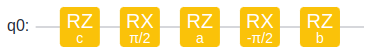
\includegraphics[width=0.9\linewidth]{images/4_1_ansatz.png}
  \end{center}
  \caption{可作为任意单量子比特旋转的 ansatz 线路。}
  \label{fig:u3_ansatz}
\end{figure}

可观测量实现如下：

\begin{lstlisting}
from mindquantum.core.operators import QubitOperator
from mindquantum.core.operators import Hamiltonian

obs = QubitOperator('X0')
ham = Hamiltonian(obs)
\end{lstlisting}

在 \MindQuantum\ 中，模拟器提供了 \getexpectationwithgrad\ 方法，可方便地计算 $E_X(\theta)$ 的梯度。

\begin{lstlisting}
import numpy as np
from mindquantum.simulator import Simulator

sim = Simulator('mqvector', ansatz.n_qubits)
grad_ops = sim.get_expectation_with_grad(ham, ansatz)

p0 = np.random.uniform(-np.pi, np.pi, len(ansatz.params_name))
f, g = grad_ops(p0)
print(f, g)
\end{lstlisting}
输出为：
\begin{lstlisting}
[[-0.04602095+0.j]] [[[-1.17340357e-17+0.j -3.47310364e-02+0.j -7.96875999e-01+0.j]]]
\end{lstlisting}

\getexpectationwithgrad\ 接收可观测量哈密顿量和 ansatz 线路，并返回一个梯度算符。可以使用该算符在任意 ansatz 参数处计算梯度。梯度算符的输出包含期望值及其关于 ansatz 参数的梯度。期望值的形状为 $[n_\text{batch}, n_\text{ham}]$，其中 $n_\text{batch}$ 是编码器数据的批大小，$n_\text{ham}$ 是哈密顿量数量。在该任务中，我们没有编码器，且只有一个可观测量，因此 $n_\text{batch}=1, n_\text{ham}=1$。ansatz 梯度的形状为 $[n_\text{batch}, n_\text{ham}, n_\text{ansatz}]$，其中 $n_\text{ansatz} = 3$ 是 ansatz 线路中的参数数量。

下一步是借助梯度算符优化 PQC。
\begin{lstlisting}
from scipy.optimize import minimize

def fun(p0, grad):
  f, g = grad(p0)
  f = np.real(f)[0, 0]
  g = np.real(g)[0, 0]
  return f, g

res = minimize(fun, p0, method='bfgs', jac=True, args=(grad_ops, ))
print('min E:', res.fun)
print('Best p:', res.x)
\end{lstlisting}
可以得到最小化后的可观测量取值以及对应的 ansatz 参数：
\begin{lstlisting}
min E: -0.9999999999994561
Best p: [-2.51566965 -4.71238798 -3.14159296]
\end{lstlisting}
因此，学习得到的旋转为：
\begin{lstlisting}
ansatz.matrix(pr=dict(zip(ansatz.params_name, res.x)))
\end{lstlisting}
\begin{align*}
  U_a=\frac{1}{\sqrt{2}}\begin{pmatrix}
    e^{-0.313i}  & e^{0.313i} \\
    -e^{-0.313i} & e^{0.313i}
  \end{pmatrix}.
\end{align*}

\subsubsection{旋转三个态}
\label{sec:rotate_three_states}

在前一个示例中，PQC 只包含 ansatz 线路；在本示例中，我们将展示如何在 \MindQuantum\ 中向 PQC 加入编码器线路。问题描述如下：寻找一个单量子比特旋转门 $U_a(\theta)$，使以下三个态的 $Z$ 期望值之和最大：$\ket{\psi_0}=\ket{0},\ket{\psi_1}=(\ket{0}+\ket{1})/\sqrt{2}$ 和 $\ket{\psi_2}=(\ket{0}+i\ket{1})/\sqrt{2}$。

\begin{equation}
  \max_{\theta}\sum_i{\bra{\psi_i}U^\dagger(\theta)ZU(\theta)\ket{\psi_i}}.
\end{equation}

这里，我们使用编码器线路 $U_e(a, b) = RX(a)RY(b)$ 制备态 $\ket{\psi_i}=U_e(a, b)\ket{0}$：
\begin{lstlisting}
import numpy as np
from mindquantum.core.circuit import Circuit

encoder = Circuit().rx('a', 0).ry('b', 0)
encoder = encoder.as_encoder()

e_data = np.array([[0.0, 0.0],      # psi_0
                   [0.0, np.pi/2],  # psi_1
                   [-np.pi/2, 0.0], # psi_2
                  ])
\end{lstlisting}
在上述代码中，我们调用 \asencoder\ 将量子线路转换为编码器线路。在本示例中，我们将展示如何借助 MindSpore 机器学习框架训练 PQC。

\begin{lstlisting}
# 构建任意单量子比特旋转 ansatz
from mindquantum.framework import MQLayer
import mindspore.nn as nn
import mindspore as ms

ansatz = Circuit().rz('a2', 0).rx(np.pi/2, 0)
ansatz.rz('a0', 0).rx(-np.pi/2, 0).rz('a1', 0)

obs = QubitOperator('Z0')
ham = Hamiltonian(-obs)

sim = Simulator('mqvector', 1)
total_circ = encoder + ansatz
grad_ops = sim.get_expectation_with_grad(ham, total_circ)

e_tensor = ms.Tensor(e_data, ms.float32)

quantum_net = MQLayer(grad_ops)

class Hybrid(nn.Cell):
    def __init__(self, quantum_net):
        super(Hybrid, self).__init__()
        self.quantum_net = quantum_net
    def construct(self, e):
        x = self.quantum_net(e)
        x = x.sum()
        return x

hybrid = Hybrid(quantum_net)
opti = nn.Adam(quantum_net.trainable_params(), learning_rate=0.1)
train_net = nn.TrainOneStepCell(hybrid, opti)
for step in range(100):
    print(-train_net(e_tensor))
\end{lstlisting}
最终学习得到的期望值之和为 1.732。此外，我们还可以在 \MindQuantum\ 中方便地展示这些量子态：

\begin{lstlisting}
import matplotlib.pyplot as plt
from mindquantum.io import BlochScene
from mindquantum.core.parameterresolver import ParameterResolver as PR

e_name = encoder.params_name
a_name = ansatz.params_name
a_data = np.array(quantum_net.weight)

init_states = [encoder.get_qs(pr=dict(zip(e_name, i))) for i in e_data]
final_states = []
for i, data in enumerate(e_data):
    pr = PR(dict(zip(e_name, data)))
    pr += PR(dict(zip(a_name, a_data)))
    final_states.append(total_circ.get_qs(pr=pr))

scene = BlochScene()
fig, ax = scene.create_scene()

for i in init_states:
    scene.add_state(ax,
        i,
        linecolor='r',
        with_proj=False)

for i in final_states:
    scene.add_state(ax,
        i,
        linecolor='g',
        with_proj=False)

plt.show()
\end{lstlisting}

\begin{figure}[ht]
  \centering
  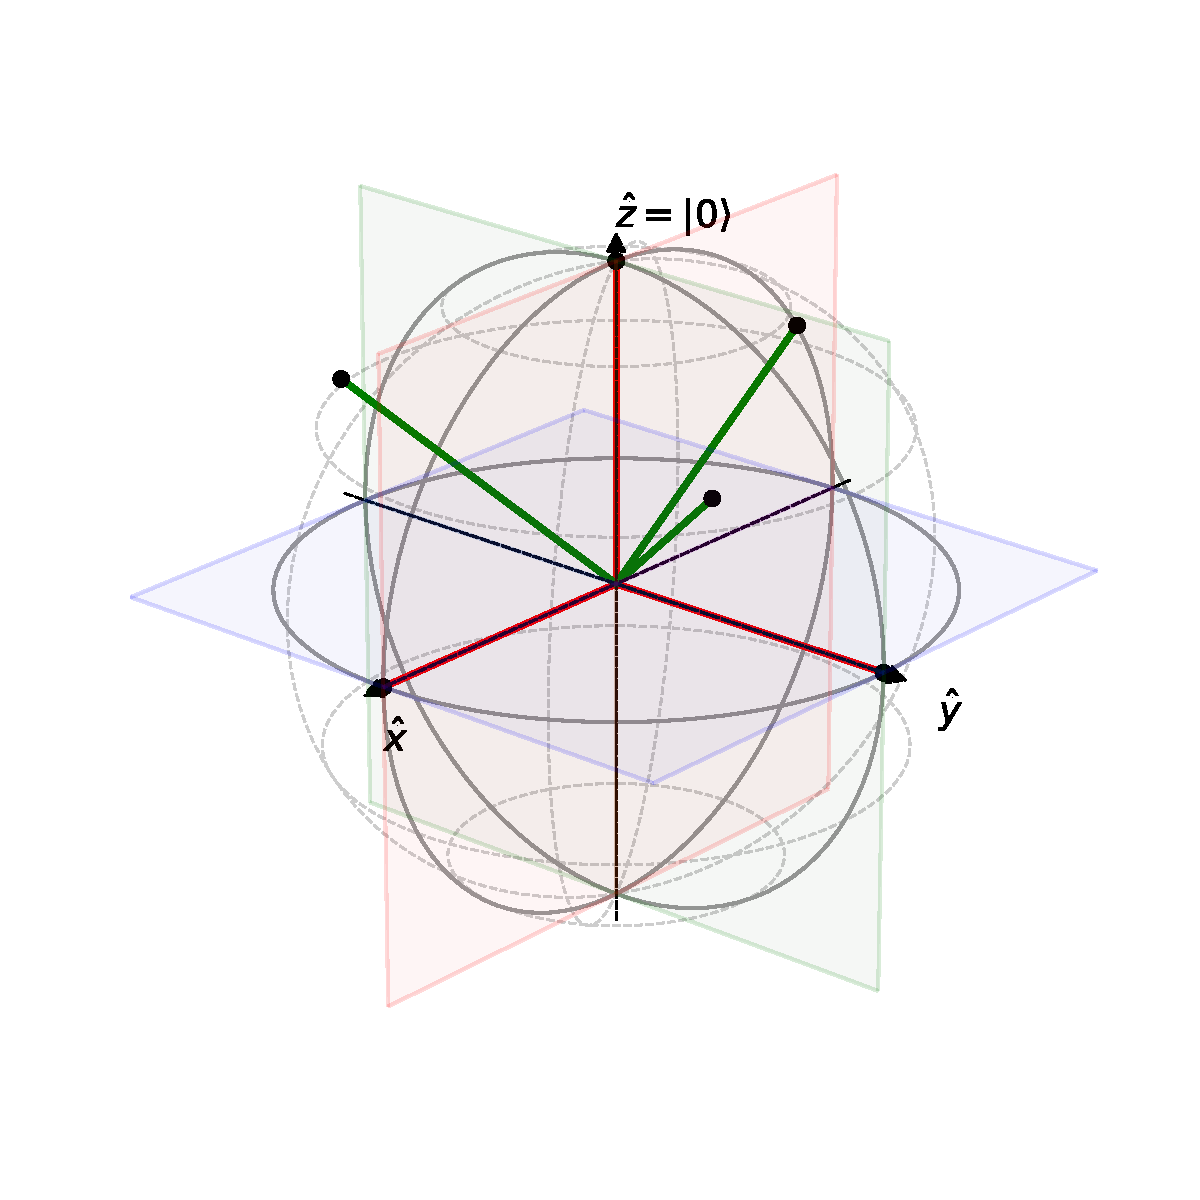
\includegraphics[scale=0.48]{./images/4_1_result.pdf}
  \caption{\label{4_1_vqa} 初始态的旋转。红色表示初始量子态，绿色表示最终量子态。}
\end{figure}

\subsubsection{更多用法}
在 \MindQuantum\ 中，除上述两种基本用法外，\getexpectationwithgrad\ 还提供了更广泛的应用场景。实际计算梯度的表达式定义为：
\begin{equation}
  E = \left<\varphi\right|U_l^\dagger H U_r \left|\psi\right>.
\end{equation}
可以将 $U_l$ 设置为空线路，并将 $H$ 设置为恒等 \QubitOperator，从而得到新态在 $\ket{\varphi}$ 上的投影。也可以设置 $\ket{\varphi}=\ket{\psi}$、$U_l = U_r$，并将 $H$ 设置为密度矩阵，例如 $H = \ket{0}\bra{0}$，此时结果为
\begin{equation}
  E=\left|\bra{0}U_r\ket{\psi}\right|^2.
\end{equation}
还可以将可观测量设置为哈密顿量列表，使 \MindQuantum\ 能够并行计算期望值和梯度。
